\begin{subappendices}
\section{Edge-disjoint K-shortest paths}
\label{sec:ksp}

For the sake of completeness, we provide a summary of the edge-disjoint K-shortest paths algorithm implemented in this work while the full version is given in~\cite{suurballe74}.
Alg.~\ref{alg:ksp} describes the pseudo code of what follows.
Given a directed acyclic graph $G$, the edge-disjoint K-shortest paths algorithm iteratively augments the set of $l$ shortest paths $P_{l}$, to obtain the optimal set $P_{l+1}$. Starting with $l=0$, we use a generic shortest-path algorithm to compute $P_0=\{p_0\}$.
In practice, we use the Bellman-Ford's algorithm \cite{bellman58}, which is adequate to cases where edges have negative costs. We then perform two kinds of transformations on $G$.

\begin{itemize}
\item[-]  {\bf{Reverse operation:}} The direction and algebraic signs of edge costs occupied by path(s) of $P_{l}$ are reversed.
\item[-] {\bf{Edge costs transform:}}
The generic shortest-paths algorithm gives for every node the cost of the shortest path from the source. We perform a cost transformation step to make all edges of our graph non-negative. This allows us to then use the more efficient Dijkstra's single source shortest path algorithm \cite{dijkstra59}, which requires non-negatives edge costs as well.
In particular, we let $v_t^n$ and $w_t^n$ be the input and output nodes of tracklets $\mathcal{T}_t^n$, and let $L(v_t^n)$ be the cost of the shortest path from the source to node $v_t^n$. We apply $\forall m,n,t$:
\begin{subequations}
\label{eq:cost_transform}
\begin{align}
&C_t^{n} \coloneqq C_t^n + L(v_t^n) - L(w_t^n)\label{eq:cost_transform_tracklet}\\
&C_{t-1}^{m,n} \coloneqq C_{t-1}^{m,n} + L(w_{t-1}^m) - L(v_{t}^n)\label{eq:cost_transform_transition}\\
&C_t^{\mathcal{E}_t,n} \coloneqq 0 \label{eq:cost_transform_entrance}\\
&C_t^{n,\mathcal{X}} \coloneqq C_t^{n,\mathcal{X}} + L(w_t^n) - L(\mathcal{X}). \label{eq:cost_transform_sink}
\end{align}
\end{subequations}
\end{itemize}

On this modified graph, we compute the interlacing path $\tilde{p}_0$. The set $P_{1}$ is obtained by {\it augmenting} $P_0$ with $\tilde{p}_0$. Concretely, we assign a negative label to the edges of $\tilde{p}_0$ that are directed towards the source, and a positive label otherwise. We then construct the optimal pair of paths $P_{1}$ by adding positive edges of $\tilde{p}$ to $P_0$ and removing negative edges from $P_0$, as shown on Fig.~\ref{fig:augment}. The next iterations follow the same procedure. Note that in general, $\tilde{p}_l$ can interlace several paths of $P_l$.

Hence, our algorithm runs Dijkstra's single source shortest path $K$ times. We therefore have a complexity time linear with $K$, \ie in a worst case scenario: $\mathcal{O} \left( K(E + V \cdot \log \, V) \right)$, with $K, V, E$ the number of path sets, nodes, and edges, respectively.

\begin{figure}[t]
\centering
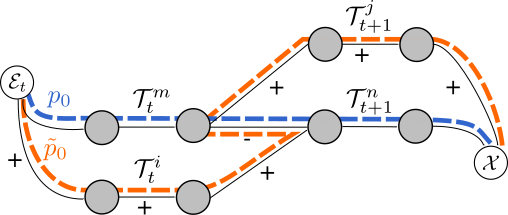
\includegraphics[width=0.49\textwidth]{figa14a}
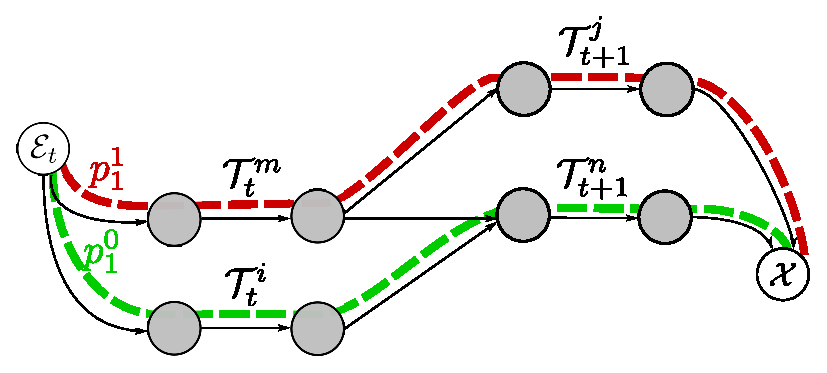
\includegraphics[width=0.49\textwidth]{figa14b}
\caption{Illustration of the interlacing and augmentation procedure for $K$=2. (Left) $p_0$ is the (single) shortest-path of set $P_0$. $\tilde{p}_0$ is the shortest interlacing path obtained after inverting the direction and algebraic sign of edge costs of $P_0$. Positive and negative labels are assigned to the edges of $P_0$. (Right) The optimal set $P_1=\{ p_1^0,p_1^1 \}$ is obtained by removing the edges with negative labels from $p_0$, and adding positive labels.}\label{fig:augment}
\end{figure}


\begin{algorithm}[t]
\caption{K-shortest paths algorithm.\label{alg:ksp}}
\begin{algorithmic}[1]
\Require{$G$: Directed Acyclic Graph constructed as in Sec.~\ref{sec:solving}}
\Ensure{$P$: Set of K-shortest paths}
\State $p_0 \gets$ \texttt{bellman\_ford\_shortest\_paths}$(G)$
\State $P_0 \gets\{p_0\} $
\For{$l\gets 0$ to $l_{max}$ }
 \If{$l \neq 0$}
   \If{\texttt{cost}$(P_l) \geq$ \texttt{cost}$(P_{l-1})$}
     \Return $P_{l-1}$
 \EndIf
 \EndIf
   \State $G_r \gets$ \texttt{reverse}$(G,P_l)$\Comment{Reverse edges directions and algebraic signs}
   \State $G_r^+ \gets$ \texttt{edge\_costs\_transform}$(G_r)$\Comment{As in Eq.~\eqref{eq:cost_transform}}
   \State $\tilde{p}_l \gets$ \texttt{dijkstra\_shortest\_paths}$(G_r^+)$\Comment{Returns interlacing path}
   \State $P_{l+1} \gets$ \texttt{augment}$(P_l, \tilde{p}_l)$\Comment{As on Fig.~\ref{fig:augment}}
\EndFor

\end{algorithmic}
\end{algorithm}
\end{subappendices}

%%% Local Variables:
%%% mode: latex
%%% TeX-master: "../../main"
%%% End:
